\documentclass[10pt, a4paper]{exam}
\usepackage{graphicx}
\usepackage[a4paper, total={7in, 9.5in}]{geometry}
\usepackage[normalem]{ulem}
\usepackage{amsmath}
\renewcommand\ULthickness{1.0pt}   
\setlength\ULdepth{1.3ex}

\begin{document}


	\noindent
	\begin{minipage}[l]{0.1\textwidth}
		\noindent
		
\includegraphics[width=2.8\textwidth]{ESCUDO.png}
	\end{minipage}
\hfill
\begin{minipage}[c]{0.8\textwidth}
	\begin{center}
		{\large  Departamento de Ingeniería civil y Agrícola\par
		\large	Facultad de Ingeniería	\par
	% \large \textbf{Taller propiedades de los fluidos}	\par
    \large \textbf{Laboratorio No. 3\\Vertedero}	\par
} Prof. Luis Alejandro Morales, Ph.D.
	\end{center}
\end{minipage}
\par
\vspace{0.2in}
\noindent
    \uline{Estructuras hidráulicas [2015954]	\hfill 2024-II	}
\par 
\vspace{0.15in}
\noindent

%%%%%%%%%%%%%%%%%%%%%%%%%%%%%
\section{Normas del Laboratorio}
\begin{itemize}
    \item \textbf{Grupos}: Los grupos serán de 5 o 6 estudiantes máximo. Los estudiantes son libres de organizar los grupos.
    
    \item \textbf{Duración}: Cada grupo tendrá una hora aproximadamente para realizar el laboratorio.
    
    \item \textbf{Material}: Es necesario vestir bata u overol para la realización del laboratorio. Este atuendo puede ser de cualquier color o fabricante. Traer calculadora, lápiz y papel.
\end{itemize}


\section{Objetivo}

En términos generales, este laboratorio tiene como fin estudiar el flujo a través de un vertedero de pared delgada con el fin de conocer y calibrar las variables que intervienen en el cálculo del caudal. Algunos objetivos específicos:

\begin{itemize}

    \item Calcular el valor del coeficiente de descarga $(C_d)$ para cada cada relaci\'on entre Q y H de acuerdo con cada tipo de vertedero. 
    
    \item Obtener la curva de patronamiento de caudal mediante diferentes métodos y comparar.
    
\end{itemize}


\section{Metodología}

Se dispondrá de un canal rectangular horizontal de paredes de vidrio de $31cm$ de ancho, dicho canal se alimenta mediante un tanque de aquietamiento que esta conectado a una tubería proveniente de un tanque de nivel constante. El caudal que pasa por el canal se regula mediante una válvula colocada en la tubería. 

El tanque volumétrico será utilizado para el cálculo del caudal que pasara por la compuerta, este valor se conoce midiendo el desplazamiento de la cinta y el tiempo que transcurre en dicho desplazamiento (Figura \ref{fig:cinta}). 

\begin{figure}[h]
    \centering
    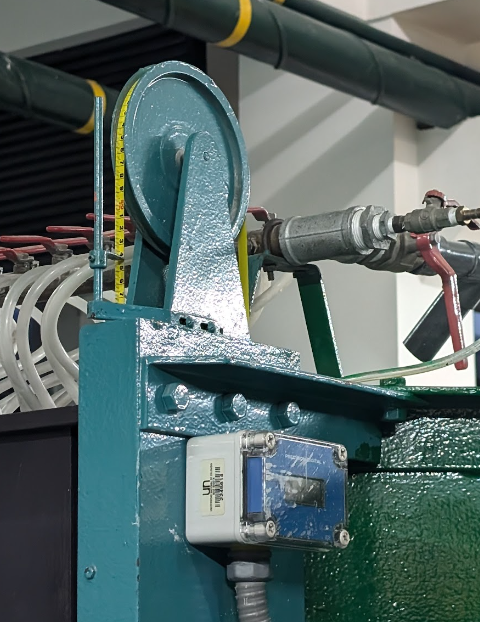
\includegraphics[width=0.29\linewidth]{Images/cinta.png}
    \caption{Cinta para la medición del caudal.}
    \label{fig:cinta}
\end{figure}

%\newpage

A lo largo del canal se encuentra un limnímetro montado en un riel desplazable a lo largo del canal. Este instrumento permite  medir  la profundidad en cualquier punto del canal. El esquemático del montaje anterior se evidencia en las imágenes \ref{fig:esqpdf}.

\begin{figure}[h]
    \centering
    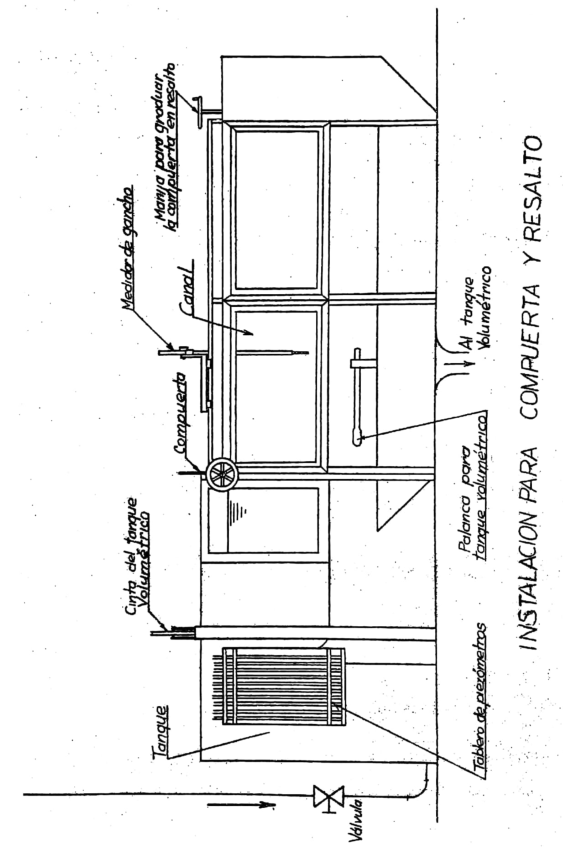
\includegraphics[angle=270,width=0.6\linewidth]{Images/esquema.png}
    \caption{Esquema general de la instalación.}
    \label{fig:esqpdf}
\end{figure}

Sobre la mitad del canal se instalarán dos tipos de vertedero de pared delgada: vertedero rectangular y vertedero triangular, para realizar la práctica (ver la figura \ref{fig:verte}):

\begin{figure}[h]
    \centering
    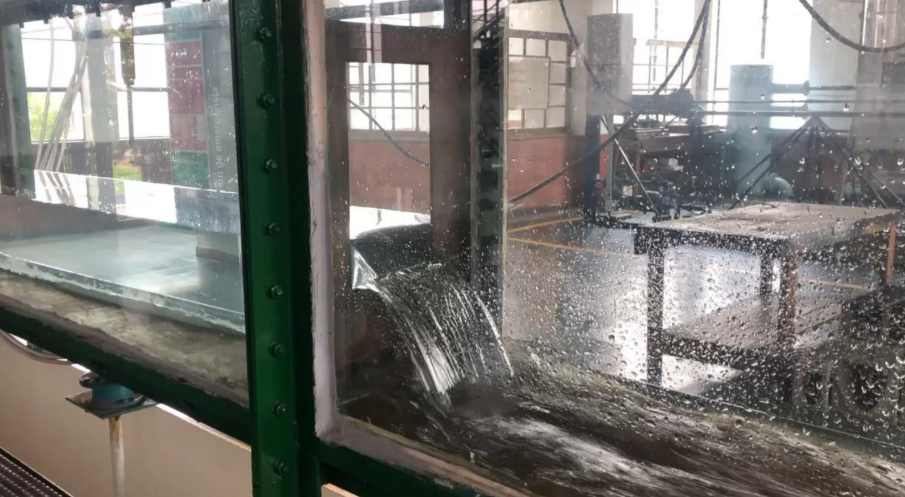
\includegraphics[width=0.7\linewidth]{Images/vertedero.png}
    \caption{Instalación de un vertedero rectangular (laboratorio de hidráulica).}
    \label{fig:verte}
\end{figure}

La fórmula general para determinar el caudal en los vertederos, cualquiera que sea su forma (rectangular, trapezoidal, triangular, parabólico, etc., o bien que sean de pared gruesa o pared delgada), es:

\begin{equation}
    Q = C_d H^n
    \label{ecu:general}
\end{equation}

Donde:  

\begin{itemize}
    \item $Q$ = Caudal 
    \item $C$ = Coeficiente de descarga
    \item $H$ = Altura de la lámina sobre la cresta del vertedero (carga).
    \item $n$ = exponente
\end{itemize}

%\newpage

\section{Ecuaciones y resultados}

\begin{enumerate}

    \item Partiendo de la ecuación general \ref{ecu:general} se obtienen las ecuaciones específicas para cada forma de vertedero, teniendo:

    \begin{itemize}
        \item \textbf{Vertedero de pared rectangular sin contracciones:} 

        \begin{equation}
            Q = \frac{2}{3} \text{Cd} \cdot L \sqrt{2g}  H^{3/2} 
            \label{ecu:vertrect}
        \end{equation}

        Donde:  

        \begin{itemize}
            \item $C_d$ = Coeficiente de descarga.
            \item $L$ = Longitud de la cresta del vertedero.
        \end{itemize}

        \item \textbf{Vertedero de pared rectangular con contracciones:} 

        \begin{equation}
            Q = \frac{2}{3} \text{Cd} \cdot L' \sqrt{2g}H^{3/2}
        \end{equation}

        Donde:  

        \begin{itemize}
            \item $L'$ = $L-0.1n$
            \item $n$ = número de contracciones laterales.
        \end{itemize}

        \item \textbf{Vertedero triangular:} 

        \begin{equation}
            Q = \frac{8}{15} \text{Cd} \tan \left(\frac{\theta}{2}\right) \sqrt{2g}  H^{5/2}
        \end{equation}

        Donde:  

        \begin{itemize}
            \item $\theta$ = ángulo del vertedero (escotadura).
        \end{itemize}

        \item \textbf{Vertedero Trapezoidal:} 

        \begin{equation}
            Q = \frac{2}{3} \text{Cd} \cdot L \sqrt{2g} H^{3/2} + \frac{8}{15}\text{Cd}  \tan \left(\frac{\theta}{2}\right) \sqrt{2g} H^{5/2}
        \end{equation}

        Note que la expresión anterior es la combinación de un vertedero rectangular y uno triangular.

        \item \textbf{Vertedero sutro o proporcional:} 

        \begin{equation}
           Q = \pi K C_d\sqrt{2gH}
        \end{equation}

        Donde:  

        \begin{itemize}
            \item $K$ = Constante de la curva.
            \item $x\sqrt{y}=K$ = Curva correspondiente a la cresta del vertedero.
        \end{itemize}


    \end{itemize}

    \item Para la medición del caudal, se toma una medición inicial con la cinta (fig \ref{fig:cinta}), y luego una final después de 90 segundos, luego la resta entre estas dos mediciones corresponderá a la medición del tanque, se recomienda tomar 4 de estas mediciones y promediarlas, de modo qué:

    $$dif.alturas_1=med_{t=0s}-med_{t=90s}=alt.final_{1}$$

    Teniendo en cuenta que el tanque es de $2.2m$ por $7.1m$ se tendrá:

    $$Q (m^3/s)=\dfrac{(2.2m\cdot 7.1m \cdot (prom.alt.final) m)}{90seg}$$

    \item Con el limnímetro se mide la carga sobre el vertedero $(H)$ para cada uno de los caudales de la práctica, se recomiendan realizar para un total del 6 caudales.

    \item Se calcula el valor de $C_d$ despejando de la ecuación \ref{ecu:vertrect} para cada valor de caudal y luego se promedian para obtener así el primer valor de $C=\frac{2}{3} \text{Cd} \cdot L \sqrt{2g}$, obteniendo así la primera ecuación del vertedero.

    \item Luego, tomando cada uno de los valores de $H$ hallados con el limnímetro y elevados a $(3/2)$, obtenga el segundo valor de C mediante una regresión lineal, obteniendo así la segunda ecuación del vertedero.

    \item Finalmente para obtener la tercera ecuación de patronamiento utilice el método de mínimos cuadrados, donde:

    $$log(Q)=log(CH^n)$$
    $$log(Q)=log(C)+nlog(H)$$

    Donde:  

        \begin{itemize}
            \item $y$ = $log(Q)$
            \item $a$ = $log(C)$
            \item $b$ = $n$
            \item $x$ = $log(H)$
        \end{itemize}

    Obteniendo una función lineal de la forma $y=bx+a$, donde $a$ y $b$ serán:

    $$a=\dfrac{\sum y\sum x^2-\sum x\sum xy}{N\cdot\sum x^2-(\sum x)^2}$$

    $$b=\dfrac{N\cdot\sum xy- \sum x\sum y}{N\cdot\sum x^2-(\sum x)^2}$$

    Donde:  

        \begin{itemize}
            \item $N$ = Número de puntos considerados (en este caso 6).
        \end{itemize}

    \item Construya una gráfica donde muestre 4 curvas, la primera corresponderá a los puntos obtenidos de $Q$ y $H$ experimentalmente, y las otras 3 correspondientes a las ecuaciones halladas en los pasos anteriores, calcule los errores y concluya.
    
\end{enumerate}


\section{Listado de instrumentos usados}

\begin{enumerate}

    \item Medición de caudal:
    
        \begin{enumerate}
        
            \item \textbf{Tanque volumétrico:} Utilizado para medir el caudal.

            \item \textbf{Vertedero de pared delgada:} estructura hidráulica utilizada para medir y controlar el caudal de un flujo de agua. Se caracteriza por tener un borde afilado o delgado sobre el cual el agua fluye en forma de lámina delgada, sin adherirse a la pared aguas abajo. Su diseño permite que el flujo sea libre y bien definido, lo que facilita la aplicación de ecuaciones hidrométricas para determinar el caudal con precisión. Este tipo de vertedero se emplea comúnmente en laboratorios de hidráulica, canales de irrigación y sistemas de drenaje.
            
        \end{enumerate}
        
    \item Medición y control de altura:
    
        \begin{enumerate}
        
            \item \textbf{Compuertas:} Utilizadas aguas arriba y aguas abajo del canal para regular el flujo.
            \item \textbf{Limnímetro:} Conjunto de reglas graduadas en centímetros que miden las variaciones del nivel de la superficie del agua.
            
        \end{enumerate}
        
\end{enumerate}

\section{Informe}

El informe de laboratorio debe contener las siguientes secciones:

\begin{enumerate}

    \item \textbf{Introducción:} Breve texto para poner en contexto el laboratorio.
    
    \item \textbf{Metodología:} Describe el procedimiento de toma de datos y el seguido para obtener los resultados (sustentar con algunas fotografías de ser posible).
    
    \item \textbf{Resultados y análisis:} Presenta los resultados del laboratorio. Dado el caso, se deben incluir gráficas y tablas que resuman los resultados.
    
    \item \textbf{Conclusiones:} Se discuten allí las conclusiones obtenidas a partir de los resultados. Se hacen las comparaciones del caso.
    
    \item \textbf{Referencias:} Incluir las referencias consultadas.
\end{enumerate}


\end{document}



